\section{Paper Overview}
% \begin{frame}{Task Objective Description}
%     \frametitle{Task Objective Description}
%     The goal of the movie dubbing task is to generate dubbing that is consistent in timbre with the reference audio and aligned with the emotions and lip movements in the movie clip.
%     \begin{itemize}
%         \item The objective is to produce dubbing that matches the timbre of the reference audio while maintaining alignment with the emotions and lip movements in the movie clip.
%         \item This requires the model to accurately pronounce words while adapting to the emotional and pacing variations in the movie clip.
%     \end{itemize}
%     \vspace{1em}
%     \textbf{Movie Dubbing Task Formula:}
%     The model generates dubbing audio that matches the original video in terms of emotion, pacing, and duration based on the reference audio, script, and reference video.
%     \begin{equation}
%         \tilde{A}_{Dub} = Model(A_{Ref}, T_s, V_{Ref})
%     \end{equation}
% \end{frame}

\begin{frame}{Task Objective Description}
    \frametitle{Task Objective Description}
    \textbf{Task Goal:} Generate dubbing that matches reference audio's timbre and aligns with movie clip's emotions and lip movements.
    \begin{itemize}
        \item \textbf{Timbre Matching:} Align with reference audio.
        \item \textbf{Emotion \& Lip Sync:} Match movie clip's emotions and lip movements.
        \item \textbf{Accurate Pronunciation:} Adapt to emotional and pacing variations.
    \end{itemize}
    \vspace{1em}
    \textbf{Task Description with Formula for Movie Dubbing Task :}
    \begin{equation}
        \tilde{A}_{Dub} = Model(A_{Ref}, T_s, V_{Ref})
    \end{equation}
\end{frame}


% \begin{frame}{Overall Method Framework Overview}
%     \frametitle{Overall Method Framework Overview}
%     The framework consists of two main training stages: Multi-Task Speaker Pre-training (MTSP) and dubbing training, which includes Prosody Consistency Learning (PCL) and Duration Consistency Reasoning (DCR) modules.
%     \begin{figure}
%         \centering
%         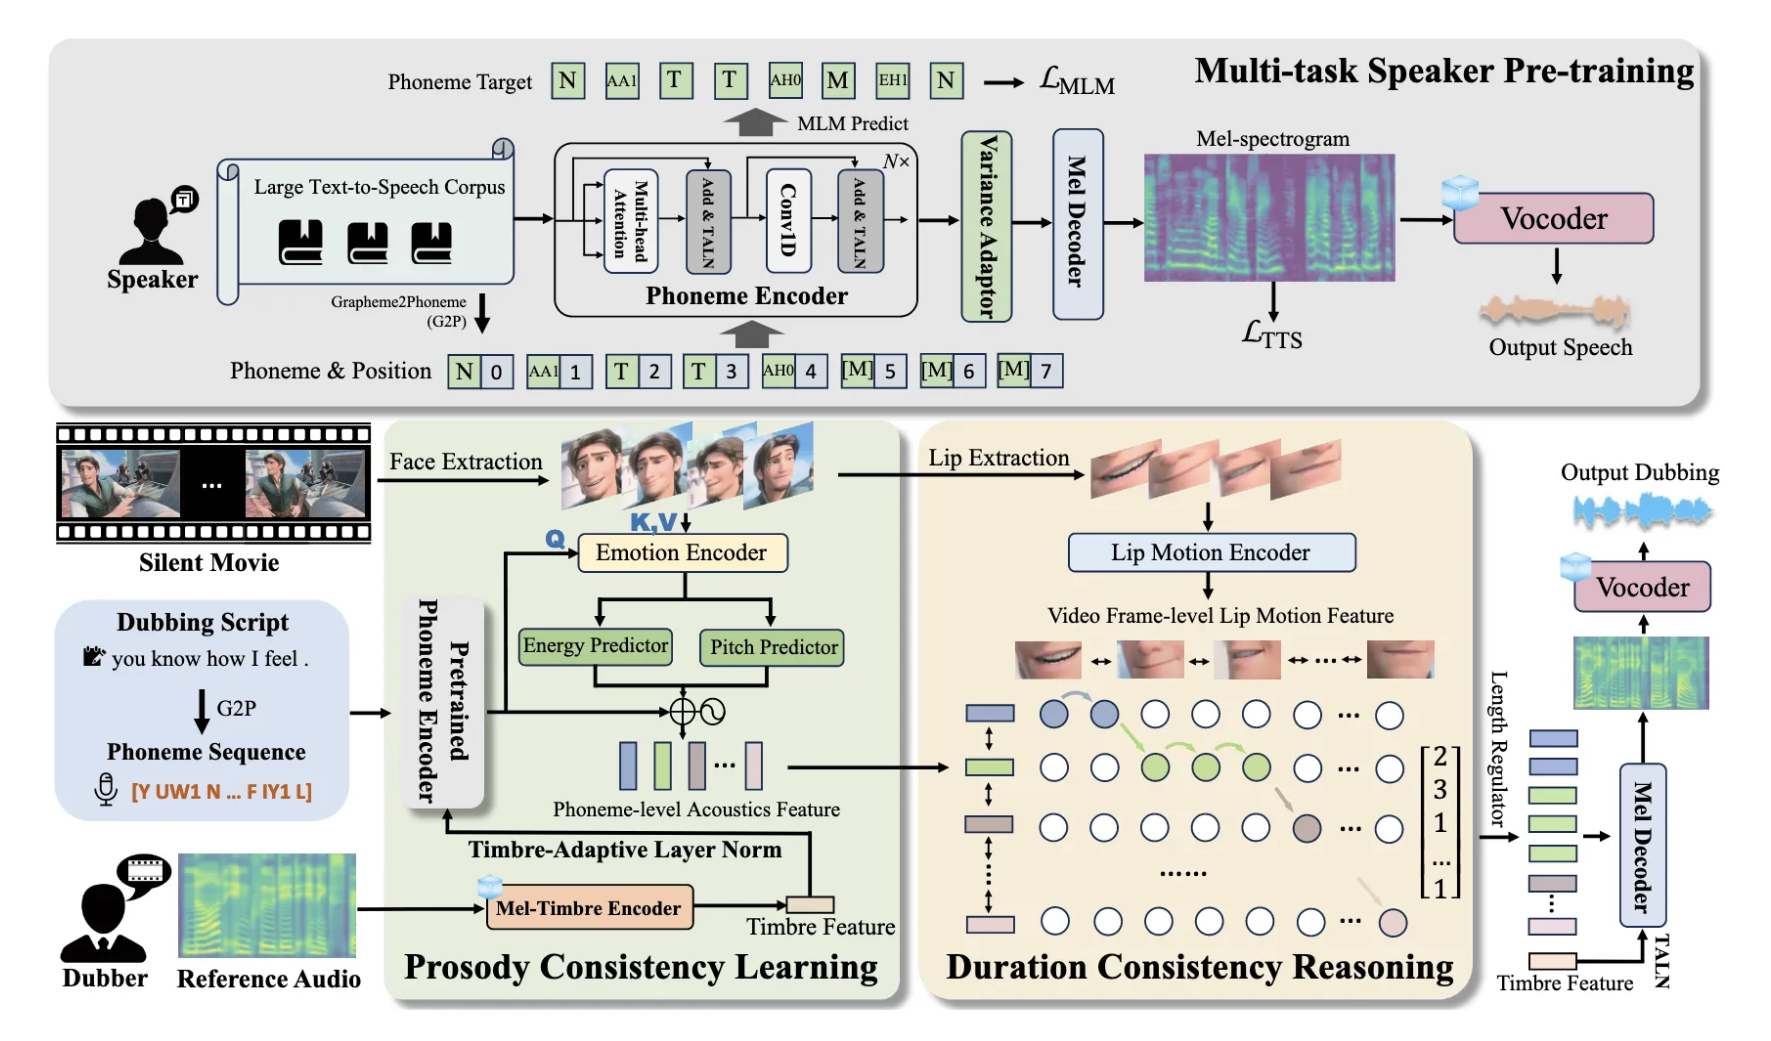
\includegraphics[width=0.6\textwidth]{figs/The main architecture.png} % Replace with your image path
%         \caption{The main architecture of the proposed two-stage dubbing method.}
%         \label{fig:method-framework}
%     \end{figure}
% \end{frame}

\begin{frame}{Overall Method Framework Overview}
    \frametitle{Overall Method Framework Overview}
    \textbf{Main Framework:}
    \begin{itemize}
        \item \textbf{MTSP:} Multi-Task Speaker Pre-training.Includes TTS task and MLM task
        \item \textbf{Dubbing Training:} Includes PCL (Prosody Consistency Learning) and DCR (Duration Consistency Reasoning).
    \end{itemize}
    \begin{figure}
        \centering
        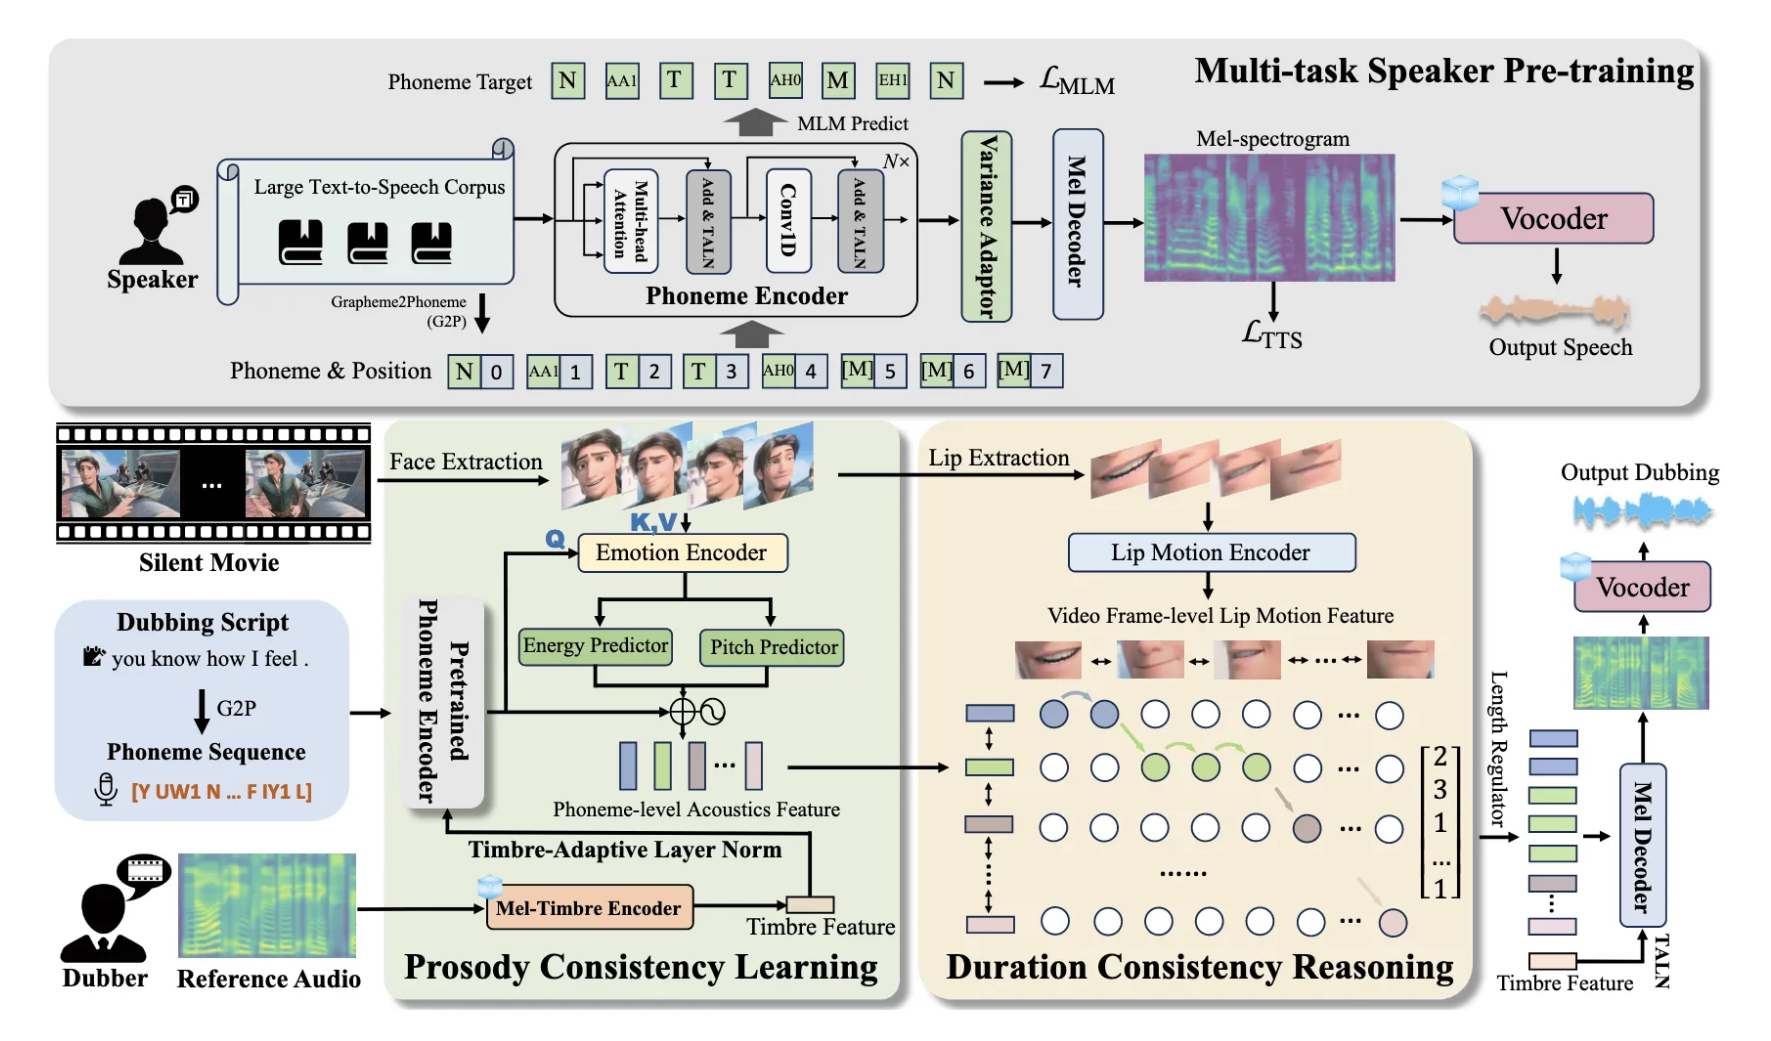
\includegraphics[width=0.45\textwidth]{figs/The main architecture.png}
        \caption{Main architecture of the two-stage dubbing method.}
        \label{fig:method-framework}
    \end{figure}
\end{frame}


% \begin{frame}{Detailed Description of the Overall Method Framework}
%     \frametitle{Detailed Description of the Overall Method Framework}
%     \begin{itemize}
%        \item \textbf{Stage 1: Multi-Task Speaker Pre-training (MTSP)}
%         \begin{itemize}
%             \item \textbf{Text-to-Speech (TTS) Task}
%             \begin{itemize}
%                 \item Objective: Learn accurate pronunciation representations from a large-scale text-to-speech corpus.
%                 \item Method: Use an architecture similar to FastSpeech2\cite{ren2020fastspeech} to predict the mel-spectrogram of the target speech.
%             \end{itemize}
%             \item \textbf{Masked Language Model (MLM) Prediction Task}
%             \begin{itemize}
%                 \item Objective: Learn contextual relationships between phonemes to better handle unseen text.
%                 \item Method: Convert text into phoneme sequences, randomly mask the sequences, and then predict the masked phoneme tokens.
%             \end{itemize}
%         \end{itemize}
%         \item \textbf{Stage 2: Dubbing Training}
%         \begin{itemize}
%             \item \textbf{Prosody Consistency Learning (PCL)}
%             \begin{itemize}
%                 \item Objective: Enhance audiovisual consistency.
%                 \item Method: Bridge the emotional states of characters in the movie clip with the phoneme-level prosody attributes of dubbing.
%             \end{itemize}
%             \item \textbf{Duration Consistency Reasoning (DCR)}
%             \begin{itemize}
%                 \item Objective: Ensure that the duration of the dubbing matches the video content.
%                 \item Method: Reason the phoneme-lip alignment and expand it to the mel length.
%             \end{itemize}
%         \end{itemize}
%     \end{itemize}
% \end{frame}

\begin{frame}{Detailed Description of the Overall Method Framework}
    \frametitle{Detailed Description of the Overall Method Framework}
    \begin{itemize}
        \item \textbf{Stage 1: Multi-Task Speaker Pre-training (MTSP)}
        \begin{itemize}
            \item \textbf{TTS Task:} Learn accurate pronunciation using FastSpeech2\cite{ren2020fastspeech} to predict target speech mel-spectrogram.
            \item \textbf{MLM Task:} Predict masked phonemes to capture phoneme context for unseen text.
        \end{itemize}
        \item \textbf{Stage 2: Dubbing Training}
        \begin{itemize}
            \item \textbf{PCL:} Enhance audiovisual consistency by aligning movie clip emotions with phoneme-level prosody.
            \item \textbf{DCR:} Ensure dubbing duration matches video content by reasoning phoneme-lip alignment.
        \end{itemize}
    \end{itemize}
\end{frame}